\documentclass[12pt]{article} %% Remove demo in your file.
\usepackage[T1]{fontenc}
\usepackage{mathptmx}  % Change this to use different font, right now this is using Times font.
\usepackage{geometry}
\usepackage{amsmath}
%\usepackage{amssymb}
%\usepackage{MnSymbol}
%\usepackage{mathabx}
%\usepackage{amsfonts}
%\usepackage{mathalpha}
\usepackage{xcolor}
\usepackage{graphicx}
\usepackage{lipsum}% Used for dummy text.
\usepackage[yyyymmdd,hhmmss]{datetime}
\usepackage{transparent}
\usepackage{tabularx}
\usepackage{multirow}
\usepackage{caption}
\captionsetup[table]{font=small,skip=0pt}
\captionsetup[figure]{font=small,skip=5pt}
\usepackage{subcaption}
\usepackage{listings}
\usepackage{hyperref}
\usepackage{cleveref}
\usepackage{natbib}
%\crefname{subsection}{subsection}{subsections}
\usepackage[acronym]{glossaries}
\hypersetup{
    colorlinks=true,
    linkcolor=blue,
    citecolor=blue,
    filecolor=magenta,
    urlcolor=magenta,
    pdfpagemode=FullScreen,
    }

% Note: You can change the layout of page and author name and other details in the title_page.tex
% file. Define a color corresponding to the BU color.
\definecolor{bured}{rgb}{0.8, 0.0, 0.0}

% A new command to insert a page without adding to the page number
\newcommand\npnpn[1]{\clearpage\thispagestyle{empty}\addtocounter{page}{-1} \ \clearpage}

\makeglossaries
\begin{document}

    \begin{titlepage}
    %\newgeometry{left=7.5cm} %defines the geometry for the titlepage
    \pagecolor{bured}
    \noindent
    \fboxsep=1mm %padding thickness for the frame
    \fboxrule=1.5pt %border thickness for the frame
    \begin{figure*}[t]
        \centering
            \begin{subfigure}{.5\textwidth}
                \begin{flushleft}
                    \hspace{-6em}
\includegraphics[height=.125\textheight]{images/BostonUni.png}
                \end{flushleft}
            \end{subfigure}%
            \begin{subfigure}{.5\textwidth}
                \begin{flushright}
                    %\vspace*{-0.5em}
                    
\includegraphics[height=.115\textheight]{images/SPTL_logo_greyscale_white.png}
                    %\fcolorbox{white}{bured}{
\includegraphics[height=.11\textheight]{
                    %images/SPTL_logo_greyscale_white.png}}
                \end{flushright}
            \end{subfigure}
        \end{figure*}
    \color{white}
    \makebox[0pt][l]{\rule{1.3\textwidth}{2pt}}
    \par
    \noindent

    \begin{center}
        \vspace{10em}
        %\hspace{-2em}
        \huge{\uppercase{Title of a report based on research we somehow got funded for!}}\\
    \end{center}

    \vskip\baselineskip

    % Begin right align text
    \begin{flushright}
        \Large{
        \textcolor{black}{Author Name}\\
        \textcolor{black}{Space Physics and Technology Lab}\\
        \textcolor{black}{Center for Space Physics}\\
        \textcolor{black}{Boston University}\\
        }
    \end{flushright}
    % Add text at the bottom of the page
    \vspace{7em}
    \begin{center}
        \vfill
        \textcolor{black}{Last updated on: \today ~@ \currenttime ~GMT}\\
        \textcolor{black}{Version: \texttt{V 0.01}}
        %\copyright{2019, Boston University}
    \end{center}
    \vfill
    \noindent

    %\clearpage\thispagestyle{empty}\addtocounter{page}{-1}
    \newpage\thispagestyle{empty}\addtocounter{page}{-1}
    \nopagecolor%
    % Add text mentioning copyright
    \vspace*{\fill}
    \begin{center}
        \textcolor{black}{\copyright{2022, Boston University}\\
        This document is the property of Space Physics and Technology Laboratory (SPTL) at Boston
        University.\\
        No part of this report may be used for commercial purposes without the express permission of
        institute and the author.}\\
    \end{center}
    \vspace*{\fill}
    \begin{figure*}[b]
        %\vspace{0.35\paperheight}
        \centering
            {\transparent{0.2}
                
\includegraphics[height=0.125\textheight]{images/sptl_v2.png}
            }%
    \end{figure*}
    \newpage
\end{titlepage}
    \nopagecolor% Use this to restore the color pages to white

    %\npnpn
    \tableofcontents
    \npnpn

    % Insert a list of figures
    \listoffigures

    % Insert a list of tables
    \listoftables
    \npnpn
    % % Include the sptl file at the bottom of the new page

    % abbreviations:
\newacronym{MSB}{MSB}{Most Significant Bit}
\newacronym{LSB}{LSB}{Least Significant Bit}
\newacronym{lexi}{LEXI}{Lunar Environment heliospheric X-ray Image}
\newacronym{met}{MET}{Mission Elapsed Time}
\newacronym{sci}{SCI}{Science Data}
\newacronym{hk}{HK}{Housekeeping Data}
\newacronym{hv}{HV}{High Voltage}
\newacronym{bu}{BU}{Boston University}
    \section[LEXI Overview]{LEXI Overview}
        \subsection[Short tile 1]{A subsection}
            The \gls{lexi} \citep{Kuntz2022} is a soft X-ray 0.1 - 2 keV) imager developed to
            provide wide field-of-view ($\sim$9.1$^{\circ}$ x 9.1$^{\circ}$) images of the
            interaction between the solar wind and Earth’s magnetosphere. The telescope will operate
            for roughly 6.5 days from the lunar surface on the Blue Ghost 1 lander from Mare
            Crisium. The project is led by \gls{bu} and is a collaboration with NASA Goddard, Johns
            Hopkins University, the University of Leicester, and the University of Miami.
            \gls{lexi} is part of NASA’s Lunar Science and Technology Program.
        \subsection[Short Title 2]{Second subsection}
            \lipsum[3-9]
            % Include a sample image
            \begin{figure}[ht]
                \centering
                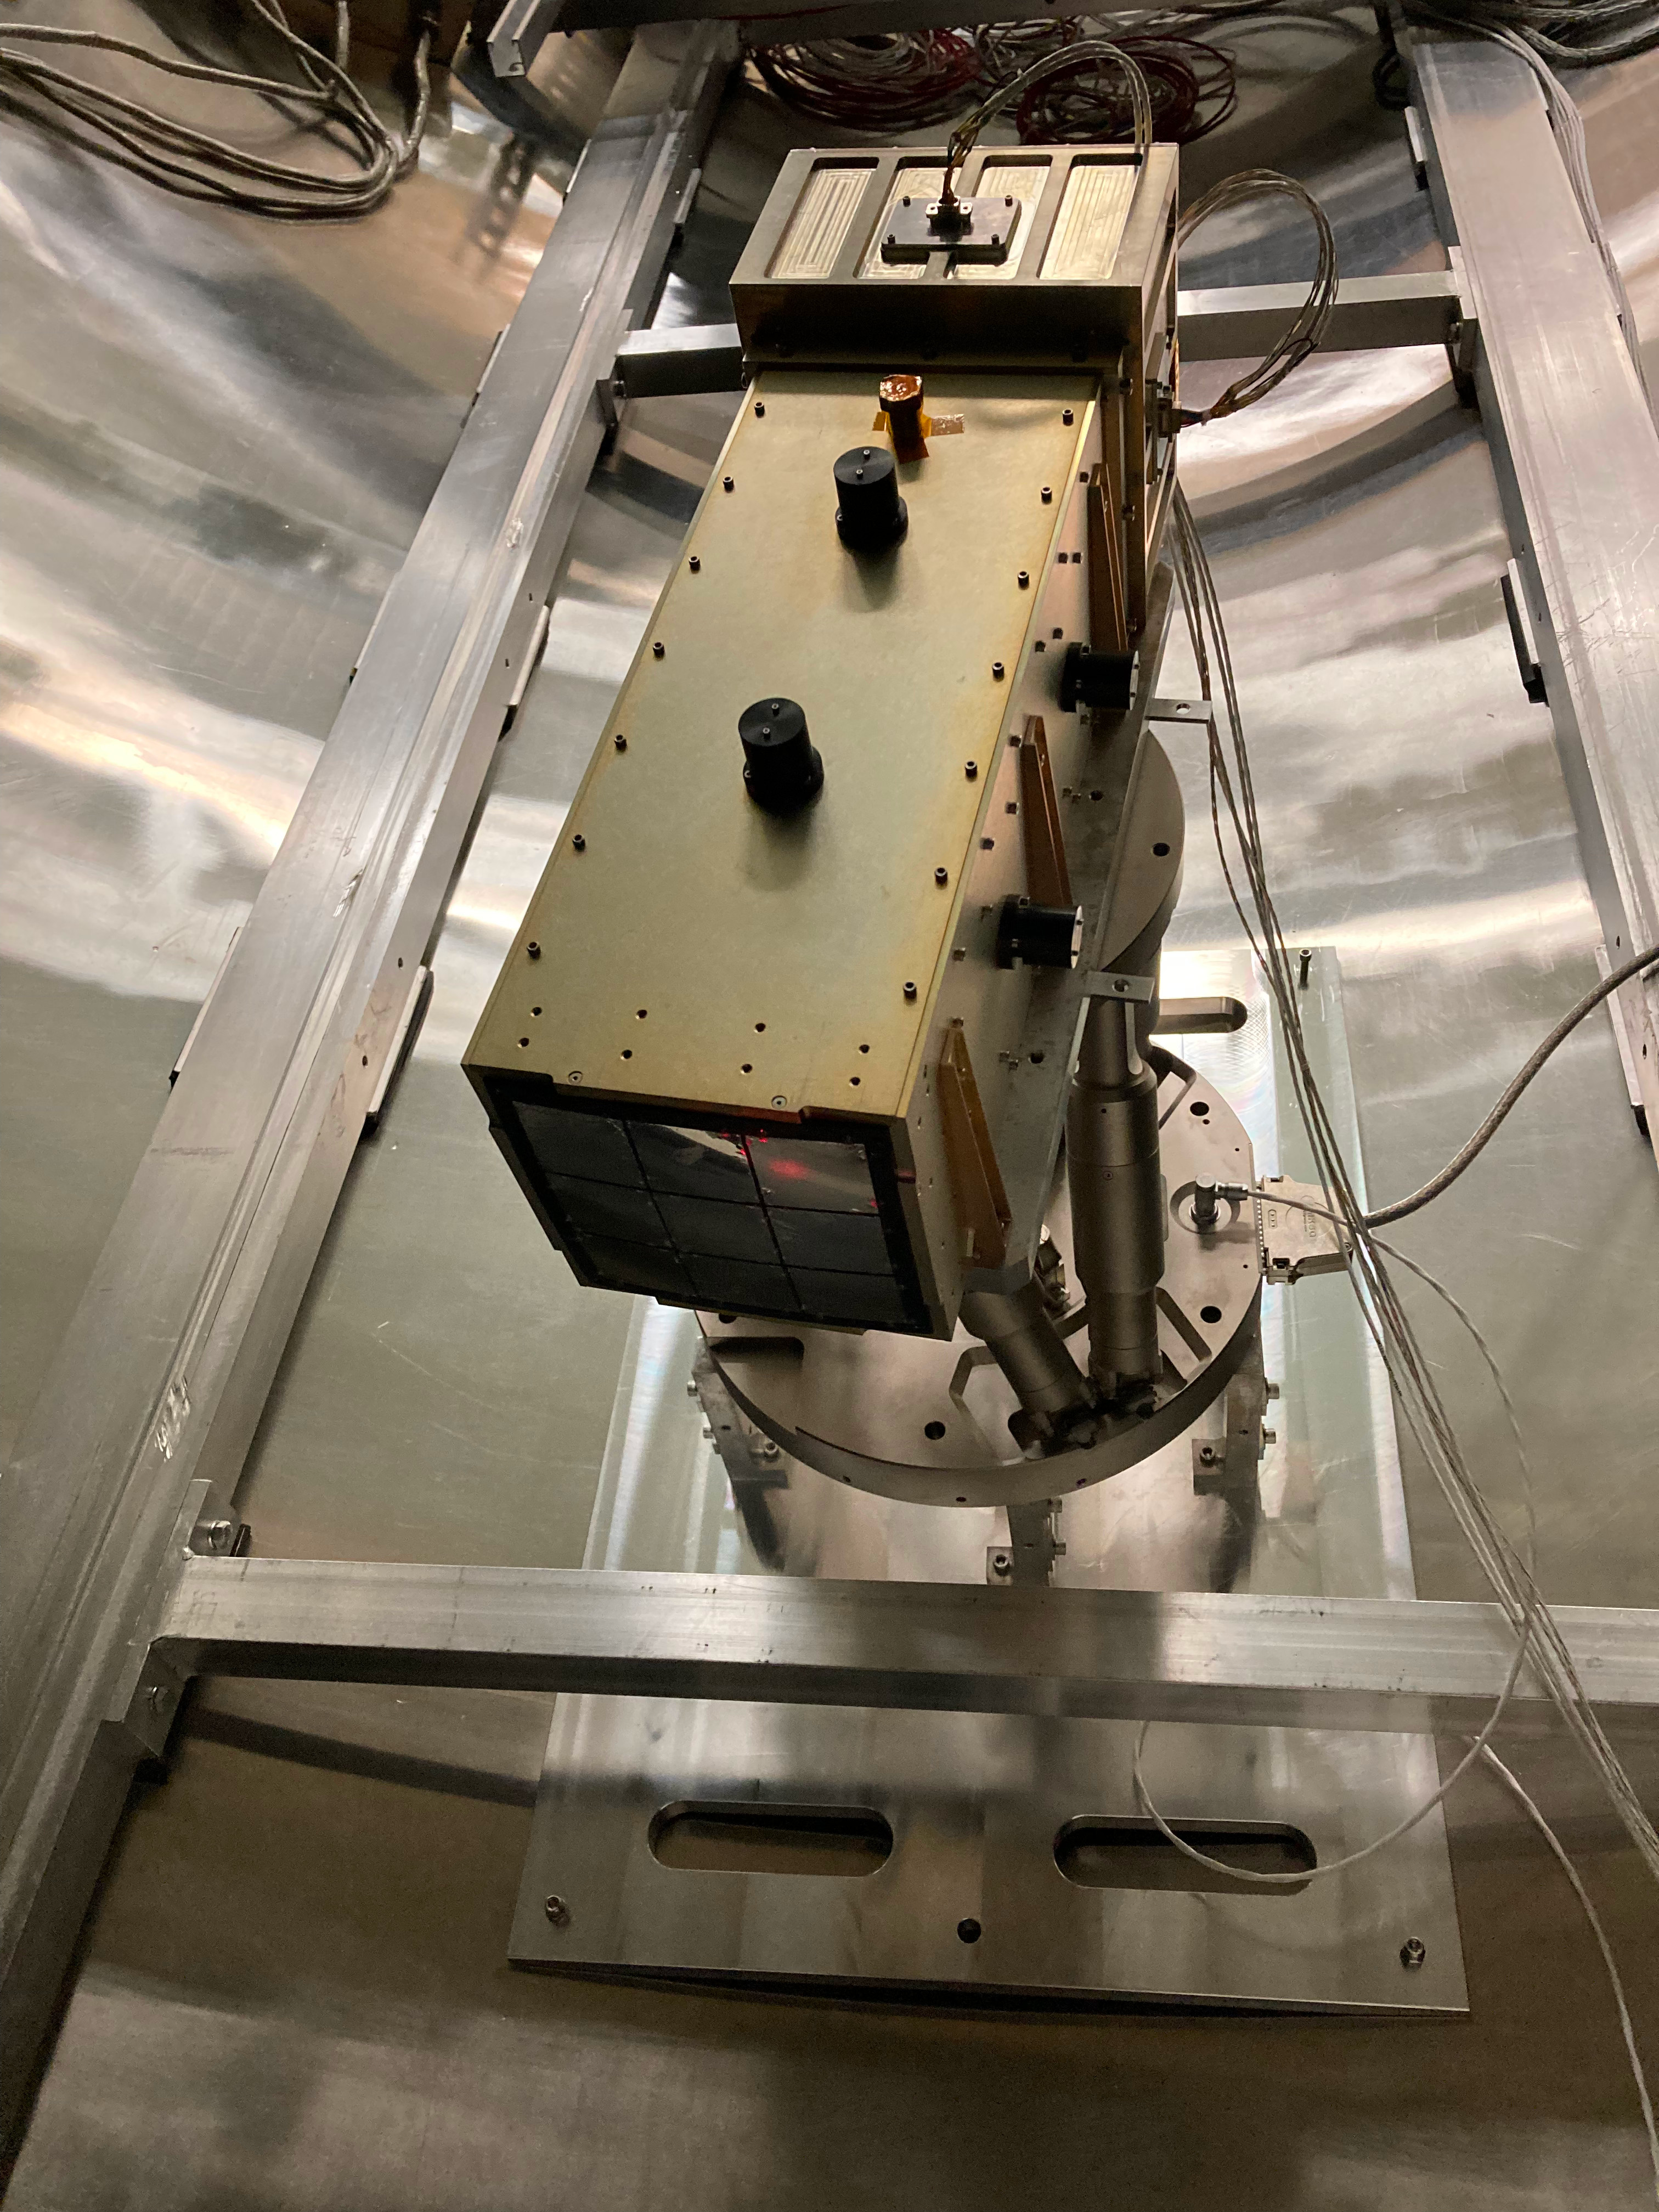
\includegraphics[width=0.5\textwidth]{images/lexi_01.jpg}
                \caption[First Fig]{This is a sample image of LEXI}
                \label{fig:lexi_01}
            \end{figure}

            % Include a sample table
            \begin{table}[ht]
                \centering
                \caption[First Table]{This is a sample table}
                \label{tab:sample_table}
                \begin{tabular}{| p {0.1\textwidth} | p {0.1\textwidth} | p {0.2\textwidth} |
                    p {0.1\textwidth} | p {0.1\textwidth} |}
                    \hline
                    \textbf{Column 1} & \textbf{Column 2} & \textbf{Column 3} & \textbf{Column 4} &
                    \textbf{Column 5} \\
                    \hline
                    \multirow{2}{*}{Row 1} & 1 & 2 & 3 & 4 \\
                    & 5 & 6 & 7 & 8 \\
                    \hline
                    \multirow{2}{*}{Row 2} & 1 & 2 & 3 & 4 \\
                    & 5 & 6 & 7 & 8 \\
                    \hline
                    \multirow{2}{*}{Row 3} & 1 & 2 & 3 & 4 \\
                    & 5 & 6 & 7 & 8 \\
                    \hline
                \end{tabular}
            \end{table}

    %
% This is the Bibliography file (bibtex.tex)
% This generally works for BibTeX

% Use sample.bib for BibTeX database
\bibliography{bibliographies/Papers}
% BibTeX style (plain, alpha, unsrt, abbrv, apalike, siam, acm, aasjournal, abbrvnat)
\bibliographystyle{aasjournal}
\nocite{}

    \printglossary[type=\acronymtype,title=Glossary of Abbreviations]
\end{document}